\chapter{Experiments}
\label{cha:experiments}
\vspace{0.4 cm}

In this chapter, we're going to delve into the experiments we've crafted to put our approach into action and assess its performance. We'll walk you through the design, implementation, and evaluation steps, providing a detailed account of each experiment. These experiments are crucial to demonstrating the effectiveness and practicality of our approach in real-world scenarios

\section{Data Collection}
\label{sec:data_collection}
\vspace{0.2 cm}
Within this sub-chapter, we will elaborate on our methodology for assembling a collection of Java projects. We outline the procedures involved in generating test cases using automated tools such as EvoSuite and Randoop\cite{noauthor_randoop_nodate}, shedding light on the meticulous steps taken to ensure comprehensive test coverage. Additionally, we will discuss the meticulous process of preparing corresponding focal methods, elucidating how we identify and associate the specific methods targeted by each test case. This step is crucial in establishing a robust foundation for subsequent analyses and evaluations within the realm of software testing and development.

\vspace{0.1 cm}
\subsection{Java Projects Selection}
\label{sec:projects_selection}
\vspace{0.1 cm}

We carefully selected four projects, as outlined in Table \ref{tab:collected_java_projects}, from the pool of publicly available GitHub Java repositories that declare an open-source license. Our selection criteria also considered popularity, with priority given to projects boasting the highest number of stars or forks. Emphasizing diversity, we aimed to cover a spectrum of project types. Here are the project selection criteria that we followed:\\
    \begin{enumerate}
        \item \textbf{Preventing Data Leakage:} To mitigate the risk of unintentional data exposure, we systematically exclude potential repositories that might be part of the pretraining data for the considered Large Language Models (LLMs). Our focus lies on projects updated within the past three years to ensure relevance.
        
        \item \textbf{Maven Compatibility:} To streamline subsequent processes, we narrow down our dataset to repositories utilizing Maven as the package manager. This decision is based on the presence of a pom.xml file at the repository root, indicating Maven usage.

        \item \textbf{Class Threshold:} We eliminate repositories with fewer than 40 classes to avoid selecting overly simplistic projects that might not offer substantial complexity.
        
        \item \textbf{Compilation Check:} Ensuring the compilability of repositories is crucial. We mandate that all dependencies be specified in the pom.xml files and selected Java version (Java 1.8). The compilation process is executed with the command 
        \begin{verbatim}
        mvn clean compile
        \end{verbatim} and repositories failing to compile are excluded. Although roughly half of the repositories compile successfully, further exploration of compilation errors might enhance compilation success rates in future endeavors.
        
        \item \textbf{Execution Check:} Similar to the compilation criterion, we require repositories to be executable in our environment. Following the selection of the Java version, we execute the command 
        \begin{verbatim}
        cd target
        java -jar <PROJECT-SNAPSHOT>.jar
        \end{verbatim}
        and retain repositories where the command succeeds. Logs are saved for future reference, and potential investigation into reasons for execution failures is left for future work.
    \end{enumerate}
From these chosen projects, encompassing a total of 388 classes, we further refined our sample by randomly selecting nine classes, totaling 87 methods. This thoughtful selection process ensures that our tool encounters a diverse range of scenarios and project structures, contributing to a more comprehensive evaluation. Further details about these chosen classes can be found in Table \ref{tab:selected_java_projects}.

\begin{table}
    \centering
    \begin{tabular}{l | l | r}
        \textbf{Project Name} & \textbf{Classes} & \textbf{Reference} \\
        \hline
        frontend-maven-plugin & 43 & \cite{sletteberg_frontend-maven-plugin_2023} \\
        javacv & 117 & \cite{noauthor_bytedecojavacv_nodate} \\
        webdrivermanager & 44 & \cite{noauthor_bonigarciawebdrivermanager_nodate} \\
        zerocode & 184 & \cite{noauthor_authorjappszerocode_nodate} \\
    \end{tabular}
\caption{Details of the collected Java projects.}
\label{tab:collected_java_projects}
\end{table}

\begin{table}
    \centering    
    \begin{tabular}{l | l | r}
        \textbf{Class Name} & \textbf{Project Name} & \textbf{Methods} \\
        \hline
        BaseSettings & javacv & 6 \\
        Parallel & javacv & 6 \\
        SeekableByteArrayOutputStream & javacv & 3 \\
        NPMInstaller & frontend-maven-plugin & 15 \\
        NodeInstaller & frontend-maven-plugin & 18 \\
        PnpmInstaller & frontend-maven-plugin & 14 \\
        CacheHandler & webdrivermanager & 4 \\
        PropertiesProviderUtils & zerocode & 4 \\
        ZerocodeCorrelationshipLogger & zerocode & 17 \\
    \end{tabular}
\caption{Summary of selected Java projects.}
\label{tab:selected_java_projects}
\end{table}

\vspace{0.1 cm}
\subsection{Test Case Generation with EvoSuite}
\label{sec:test_case_generation}
\vspace{0.1 cm}

Our tool is designed to enhance existing test cases by focusing on improving assertions. To achieve this, we require one or more test suites, and for our research, we've opted to use EvoSuite. EvoSuite\cite{noauthor_evosuite_nodate} is a sophisticated tool specifically tailored for automatically generating test cases with assertions for Java code. It employs a unique hybrid approach that not only generates but also optimizes entire test suites to fulfill specific coverage criteria. These criteria guide the tool in producing comprehensive test suites that effectively cover the targeted code. EvoSuite doesn't stop at merely generating tests; it goes a step further by suggesting potential oracles for these test cases. Oracles, in this context, are sets of assertions strategically added to succinctly summarize the current behavior of the code. These assertions serve a crucial role—enabling developers to identify deviations from expected behavior and capturing the existing behavior to safeguard against potential defects in the future.

For our study, we utilized EvoSuite to generate automated test cases for each of the selected classes. We adhered to the default configurations of EvoSuite, setting the search budget to 15 and opting not to minimize. We generated 9 Test Suites with a total of 138 test cases. The generated test suites for each class are outlined in Table \ref{tab:evosuite_testclasses}.

\begin{table}
    \centering    
    \begin{tabular}{l | l | r}
        \textbf{Test Suite} & \textbf{Class Name} & \textbf{Test Cases} \\
        \hline
        BaseSettings\_ESTest & BaseSettings & 14 \\
        Parallel\_ESTest & Parallel & 6 \\
        SeekableByteArrayOutputStream\_ESTest & SeekableByteArrayOutputStream & 13 \\
        NPMInstaller\_ESTest & NPMInstaller & 18 \\
        NodeInstaller\_ESTest & NodeInstaller & 18 \\
        PnpmInstaller\_ESTest & PnpmInstaller & 21 \\
        CacheHandler\_ESTest & CacheHandler & 13 \\
        PropertiesProviderUtils\_ESTest & PropertiesProviderUtils & 14 \\
        ZerocodeCorrelationshipLogger\_ESTest & ZerocodeCorrelationshipLogger & 21 \\
    \end{tabular}
\caption{Summary of EvoSuite generated test classes.}
\label{tab:evosuite_testclasses}
\end{table}

\vspace{0.1 cm}
\subsection{Metadata Extraction}
\label{sec:data_extraction}
\vspace{0.1 cm}

This step involves parsing each project to extract essential information about classes and methods, along with their associated metadata. Once this information is obtained, our focus shifts to identifying test classes and establishing their connections with corresponding focal classes. This pivotal step ensures that we precisely match each test class with its relevant counterpart. Following the identification of test classes and their associations, we move on to a crucial mapping process. For every test case within a test class, we meticulously map it to the corresponding focal method. This meticulous mapping results in a comprehensive set of mapped test cases, forming the foundation for subsequent stages in our methodology.

\begin{itemize}
  \item \textbf{Parsing:} In the parsing phase, we thoroughly analyze each project using the tree-sitter parser\cite{noauthor_tree-sitterintroduction_nodate}. This process involves extracting valuable metadata linked to the identified classes and methods within the project. The collected information encompasses crucial details like class names, signatures, super class, bodies, annotations, interfaces, package, imports, fields, arguments list, constructors, dependencies and variables, method names, return types, any developer written comments. This parsed code serves a dual purpose: firstly, to pinpoint test cases and their corresponding focal methods, and secondly, to enhance the focal methods by incorporating focal context information.
                                
  \item \textbf{Identify Test Classes:} In this stage, our goal is to locate all the test classes within the project. Test classes are those classes housing at least one method annotated with the \textit{\textbf{@Test}} annotation. This specific annotation serves as an indicator to JUnit, signaling that the attached method is eligible to be executed as a test case. By identifying and marking classes in this manner, we establish a clear distinction between regular classes and those instrumental to the testing process. This categorization allows a systematic approach to handling test-related components.

  \item \textbf{Identify Focal Classes:} Identifying Focal Classes involves determining the class under test for each test class. We employ a two-step approach using the following heuristics:
        \begin{enumerate}
            \item \textbf{Extracting Class Instances:} The initial heuristic involves analyzing each test method to identify all the classes instantiated or any objects created during the testing process.
            \item \textbf{Matching Class Names:} Subsequently, we employ name matching as the second heuristic. Test classes typically follow a naming convention that includes the name of the focal class, often with a \textit{"Test"} prefix or suffix. For instance, a test class associated with the \textit{"BaseSettings.java"} class might be named \textit{"BaseSettingsTest.java"} or, in the case of Evosuite, \textit{"BaseSettings\_ESTest.java."} To identify the focal class, we perform name matching by comparing the name of the test class (minus the optional \textit{"\_ESTest"} suffix) with potential focal classes. This step ensures a robust association between test classes and their corresponding focal classes.
        \end{enumerate}

  \item \textbf{Identify Focal Method:} Determining the focal method for each test case involves employing specific heuristics. 
  \begin{enumerate}
      \item \textbf{Matching Method Names:} This heuristic leverages the common practice of naming test cases similarly to their corresponding focal methods. This involves matching test case names with focal methods, considering potential prefixes or suffixes like "Test."
      \item \textbf{Analyzing Method Invocations:} Additionally, this heuristic is applied if the initial method doesn't identify a focal method. We try to match the last method invocation before (or within) the assert statement within the test case and the methods defined in the focal class. If a match is found, it is selected as the focal method. We also collect other method invocations as it might be useful to prepare the focal context. This approach is grounded in the confidence gained from prior matching of the test class to the focal class, making it likely that the test case is specifically targeting that single method.
  \end{enumerate}

  Following these heuristics, we obtain a set of test cases paired with their corresponding focal class and focal methods. Test cases where we couldn't identify the focal method using our heuristics are excluded from further consideration.
  
\end{itemize}

\section{Preprocessing}
\label{sec:preprocessing}
\vspace{0.2 cm}

The EvoOracle's prompt processor component employs a two-step approach using specific heuristics to preprocess test cases, ensuring they are appropriately prepared for prompt generation. We used the regex pattern shown in Listing~\ref{assertions_regex} for both the following steps:

    \begin{enumerate}
        \item \textbf{Removal of Assertions:} All selected test cases undergo the removal of assertions, retaining only the last assertion in case there are multiple assertions using Algorithm~\ref{algorithm_remove_assertion}. This decision is based on the likelihood that reaching the last assertion implies satisfaction of all preceding assertions. This is a reasonable choice which is also seen in the work of Tufano et al. \cite{tufano_generating_2022}. The purpose is to streamline the test cases for further processing.

        \item \textbf{Placeholder Insertion:} Following the removal of additional assertions, the test cases are left with a single assertion. We replace this single assertion with \textit{"\_\_ASSERTION\_PLACEHOLDER\_\_"} placeholder using Algorithm~\ref{algorithm_placeholder_insertion}. This placeholder serves as a temporary marker and will be subsequently replaced with assertions generated by the Large Language Models.
    \end{enumerate}

    %Assertion selection Regex highlighting
    \hrule
    \begin{lstlisting}[language=Python, caption=Assertion selection Regex, label=assertions_regex]
    assertion_patterns = [
        r'(\w+\.)?assert\s*\(.+?\);',           # Matches ClassName.assert(...)
        r'(\w+\.)?assertTrue\s*\(.+?\);',       # Matches ClassName.assertTrue(...)
        r'(\w+\.)?assertNull\s*\(.+?\);',       # Matches ClassName.assertNull(...)
        r'(\w+\.)?fail\s*\(.+?\);',             # Matches ClassName.fail(...)
        r'(\w+\.)?assertFalse\s*\(.+?\);',      # Matches ClassName.assertFalse(...)
        r'(\w+\.)?assertNotEquals\s*\(.+?\);',  # Matches ClassName.assertNotEquals(...)
        r'(\w+\.)?assertEquals\s*\(.+?\);',     # Matches ClassName.assertEquals(...)
        r'(\w+\.)?assertArrayEquals\s*\(.+?\);',# Matches ClassName.assertArrayEquals(...)
        r'(\w+\.)?assertNotNull\s*\(.+?\);',    # Matches ClassName.assertNotNull(...)
        r'(\w+\.)?assertNotSame\s*\(.+?\);',    # Matches ClassName.assertNotSame(...)
        r'(\w+\.)?assertSame\s*\(.+?\);',       # Matches ClassName.assertSame(...)
        r'(\w+\.)?assertThat\s*\(.+?\);',       # Matches ClassName.assertThat(...)
    ]
    \end{lstlisting}
    \hrule
    
    \begin{algorithm}
    \caption{Algorithm for \texttt{Removing all assertions but last}}
    \label{algorithm_remove_assertion}
    \begin{algorithmic}[1]
    \Function{remove\_all\_assertions\_but\_last}{$\text{source\_code}$}
        \State $\text{assertion\_patterns} \gets$ [\texttt{...}] \Comment{List of assertion patterns}
        \State $\text{assertions} \gets \text{re.findall(assertion\_pattern, source\_code)}$
    
        \If{\text{not assertions}}
            \State \textbf{return} $\text{source\_code}$
        \EndIf
    
        \State $\text{replaced\_assertions} \gets []$
    
        \For{$i$ \textbf{in} \text{range}(\text{len(assertions) - 1})}
            \State $\text{source\_code} \gets \text{re.sub(assertion\_pattern, "", source\_code, count=1)}$
            % \State $\text{replaced\_assertions.append(assertions[i][0] + assertions[i][1] + "();")}$  % Uncomment this line if you want to keep track of removed assertions
        \EndFor
    
        \State \textbf{return} $\text{source\_code}$
    \EndFunction
    \end{algorithmic}
    \end{algorithm}

    \begin{algorithm}
    \caption{Algorithm for \texttt{Placeholder insertion}}
    \label{algorithm_placeholder_insertion}
    \begin{algorithmic}[1]
    \Function{replace\_assertions}{$\text{source\_code}$}
        \State $\text{assertion\_patterns} \gets$ [\texttt{...}] \Comment{List of assertion patterns}
        \State $\text{replaced\_assertions} \gets$ [] \Comment{List to store replaced assertions}
    
        \For{$\text{pattern}$ \textbf{in} $\text{assertion\_patterns}$}
            \Function{replacement}{$\text{match}$}
                \State $\text{matched\_text} \gets \text{match.group(0)}$
                \State $\text{replaced\_assertions.append(matched\_text)}$
                \State \textbf{return} \texttt{(ASSERTION\_PLACEHOLDER)}
            \EndFunction
    
            \State $\text{source\_code} \gets \text{re.sub(pattern, replacement, source\_code)}$
        \EndFor
    
        \State \textbf{return} $\text{source\_code, replaced\_assertions}$
    \EndFunction
    \end{algorithmic}
    \end{algorithm}
        
\section{Large Language Model Integration}
\label{sec:llm_integration}
\vspace{0.2 cm}

To improve the Oracles generated by the automated test generation tools, we propose the inclusion of LLMs into the test generation process. Recognizing that LLMs typically demand substantial resources and powerful hardware, we opted to leverage GPT4All~\cite{noauthor_gpt4all_nodate} to make this solution accessible to developers on standard development machines.

\textbf{GPT4All:} The GPT4All~\cite{noauthor_gpt4all_nodate} project, initiated by Nomic AI, seeks to democratize access to Large Language Models by enabling training and deployment on common hardware. This open-source ecosystem facilitates the integration of LLMs into applications without the need for costly platform subscriptions or specialized hardware. Notably, GPT4All addresses accessibility by providing pretrained models with reduced sizes, ensuring they can operate efficiently on CPUs, even on PCs lacking internet connectivity or a GPU. This innovation allows smaller entities and independent researchers to harness LLMs for various applications, such as content creation, coding, document comprehension, and information retrieval. With a user-friendly one-click installer, GPT4All streamlines the process, making LLM utilization feasible on modern PCs with 4–16GB of RAM, a substantial reduction compared to traditional requirements, thanks to neural network quantization~\cite{han_deep_2016}.

\vspace{0.1 cm}
\subsection{LLM Selection and Configuration}
\label{sec:llm_configurations}
\vspace{0.1 cm}

In this subsection, an overview of ...

\vspace{0.1 cm}
\subsection{Prompt Preparation}
\label{sec:prompt_preparation}
\vspace{0.1 cm}

In this subsection, ...

\vspace{0.1 cm}
\subsection{Generating Assertions}
\label{sec:generating_assertions}
\vspace{0.1 cm}

In this subsection, ...

\vspace{0.1 cm}
\subsection{Evaluating Response Quality}
\label{sec:evaluating_response}
\vspace{0.1 cm}

In this subsection, ...

\section{Test Case Preparation}
\label{sec:test_case_preparation}
\vspace{0.2 cm}

In this section, ...

\vspace{0.1 cm}
\subsection{Assertion Integration}
\label{sec:assertion_integration}
\vspace{0.1 cm}

In this subsection, ...

\vspace{0.1 cm}
\subsection{Test Case Compilation}
\label{sec:test_compilation}
\vspace{0.1 cm}

In this subsection, an overview of ...

\vspace{0.1 cm}
\subsection{Test Case Execution}
\label{sec:test_execution}
\vspace{0.1 cm}

In this subsection, an overview of ...

\vspace{0.1 cm}
\subsection{Mutation Testing Execution}
\label{sec:mutation_testing_execution}
\vspace{0.1 cm}

To evaluate the generated tests, we use PIT\cite{noauthor_pit_nodate}. PIT is a mutation testing tool that evaluates the robustness of a test suite by introducing mutations (faults) into the source code and assessing whether the tests can detect these mutations.

\vspace{0.1 cm}
\subsection{Report Parsing}
\label{sec:report_parsing}
\vspace{0.1 cm}

When we execute mvn pit test, it triggers the generation of Mutation Coverage reports as artifacts. These reports provide valuable insights into the effectiveness of our test suite. To extract meaningful information, we begin by parsing the HTML reports generated by PIT. By parsing the HTML reports, we extract detailed information on line coverage, mutation coverage, and test strength for all tests associated with a particular class. This information is essential for evaluating the thoroughness and fault-detection capability of our test suite.

\section{Experimental Setup}
\label{sec:experimental_setup}
\vspace{0.2 cm}

For our experimental setup, we conducted the experiments on a dedicated High-Performance Computing (HPC) cluster equipped with four nodes. Each node features Intel Xeon CPU 6226R\cite{noauthor_intel_nodate} processors running at 2.9GHz, with a configuration of 32 CPUs and 16GB of RAM. To ensure consistency and reproducibility, we created a specialized Singularity\cite{noauthor_introduction_nodate} image tailored for our implemented tool, enabling seamless execution on the HPC cluster. This configuration allowed us to leverage the cluster's computational capabilities effectively for our experimentation.

\vspace{0.1 cm}
\subsection{Pre-processing}
\label{sec:preprocessing_ev}
\vspace{0.1 cm}

In this subsection, an overview of ...

\vspace{0.1 cm}
\subsection{Evaluation Metrics}
\label{sec:evaluation_metrics}
\vspace{0.1 cm}

    \begin{enumerate}
        \item \textbf{Coverage Metrics:}
        \begin{itemize}
            \item \textbf{Line Coverage:} This metric measures the proportion of lines of code that are executed by the test suite. It gives an overview of how much of the code is exercised during testing.
            \item \textbf{Mutation Coverage:} PIT introduces mutations into the code and analyzes how many of these mutations are detected by the test suite. Mutation coverage reflects the ability of tests to identify and handle different types of faults.
            \item \textbf{Test Strength:} This is a comprehensive metric that considers both line coverage and mutation coverage. It provides a holistic view of how well the tests exercise the code and how effective they are at detecting mutations.
        \end{itemize}
    \end{enumerate}

    In addition to coverage, we present five count metrics to quantify the number of test cases at specific stages of the pipeline:

    \begin{enumerate}
        \item \textbf{Unique:} Count of test cases after removing duplicates.
        \item \textbf{Parsable:} Count of test cases adhering to the Java grammar, measured both absolutely and relative to the Unique count.
        \item \textbf{Compilable:} Count of test cases that successfully compiled in their scaffolding without errors, measured both absolutely and relative to the Unique count.
        \item \textbf{Executable:} Count of test cases that were executed without errors, measured both absolutely and relative to the Unique count.
        \item \textbf{Correct:} Count of test cases that were executed without errors and invoked the correct Method Under Test (MUT), measured both absolutely and relative to the Unique count. 
    \end{enumerate}
    This metric is adopted from Tufano et al. \cite{tufano_unit_2021} and provides direct comparability, despite being computed on different repositories.

\section{Research Questions}
\label{sec:research_questions}
\vspace{0.2 cm}

In this section, we will discuss the research questions which are as follows:
\begin{itemize}
  \item RQ1: How effective the LLMs are to generate test Oracles?
  \item RQ2: How efficient the LLMs are to generate test Oracles?
\end{itemize}

\section{Results}
\label{sec:results}
\vspace{0.2 cm}

In this section, a brief introduction to ... 

\vspace{0.1 cm}
\subsection{RQ1: Effectiveness of LLMs}
\label{sec:results_rq1}
\vspace{0.1 cm}

In this subsection, an overview of ...




\begin{table}[H]
\centering

\begin{tabular}{| l | r | r | r | r | r | r |}
\hline
\multirow{2}{*}{\textbf{Class}} & \multirow{2}{*}{\textbf{EvoSuite}} & \multicolumn{5}{c|}{\textbf{EvoOracle}} \\ % Fix multicolumn formatting
\cline{3-7} % Add a horizontal line between the headers
 &  & \textbf{MPT-7B} & \textbf{Nous} & \textbf{Orca} & \textbf{Stable} & \textbf{WizardLM} \\
 &  &  & \textbf{hermes-13b} & \textbf{mini\_13B} & \textbf{Vicuna-13B} & \textbf{13B-V1.1} \\
\hline
\scriptsize\textsc{} &  &  &  &  &  &  \\
\scriptsize\textsc{BaseSettings} & 100\% & 92.75\% & 98.55\% & 85.51\% & 0\% & 21.74\% \\
\hline
\scriptsize\textsc{} &  &  &  &  &  &  \\
\scriptsize\textsc{CacheHandler} & 51.52\% & 0\% & 45.45\% & 38.38\% & 0\% & 24.24\% \\
\hline
\scriptsize\textsc{} &  &  &  &  &  &  \\
\scriptsize\textsc{NPMInstaller} & 46.49\% & 6.14\% & 19.3\% & 2.05\% & 6.14\% & 6.14\% \\
\hline
\scriptsize\textsc{} &  &  &  &  &  &  \\
\scriptsize\textsc{NodeInstaller} & 53.04\% & 25.97\% & 40.51\% & 14.18\% & 0\% & 11.97\% \\
\hline
\scriptsize\textsc{} &  &  &  &  &  &  \\
\scriptsize\textsc{Parallel} & 100\% & 21.14\% & 94.31\% & 0\% & 82.93\% & 86.18\% \\
\hline
\scriptsize\textsc{} &  &  &  &  &  &  \\
\scriptsize\textsc{PnpmInstaller} & 41.53\% & 19.21\% & 25.99\% & 11.02\% & 3.67\% & 10.17\% \\
\hline
\scriptsize\textsc{Properties} &  &  &  &  &  &  \\
\scriptsize\textsc{ProviderUtils} & 57.14\% & 38.09\% & 40.47\% & 25\% & 0\% & 47.62\% \\
\hline
\scriptsize\textsc{} &  &  &  &  &  &  \\
\scriptsize\textsc{ResolutionCache} & 18.92\% & 18.92\% & 18.92\% & 6.31\% & 18.92\% & 18.92\% \\
\hline
\scriptsize\textsc{SeekableByte} &  &  &  &  &  &  \\
\scriptsize\textsc{ArrayOutputStream} & 100\% & 12.5\% & 66.67\% & 18.75\% & 31.25\% & 43.75\% \\
\hline
\scriptsize\textsc{Zerocode} &  &  &  &  &  &  \\
\scriptsize\textsc{Correlationship} &  &  &  &  &  &  \\
\scriptsize\textsc{Logger} & 91.38\% & 36.21\% & 83.91\% & 1.15\% & 0\% & 52.87\% \\
\hline

\end{tabular}
\caption{Average Line Coverage by Class and Models.}
\label{tab:line_coverage}
\end{table}

\begin{table}[H]
\centering

\begin{tabular}{| l | r | r | r | r | r | r |}
\hline
\multirow{2}{*}{\textbf{Class}} & \multirow{2}{*}{\textbf{EvoSuite}} & \multicolumn{5}{c|}{\textbf{EvoOracle}} \\ % Fix multicolumn formatting
\cline{3-7} % Add a horizontal line between the headers
 &  & \textbf{MPT-7B} & \textbf{Nous} & \textbf{Orca} & \textbf{Stable} & \textbf{WizardLM} \\
 &  &  & \textbf{hermes-13b} & \textbf{mini\_13B} & \textbf{Vicuna-13B} & \textbf{13B-V1.1} \\
\hline
\scriptsize\textsc{} &  &  &  &  &  &  \\
\scriptsize\textsc{BaseSettings} & 53.33\% & 13.33\% & 37.78\% & 20\% & 0\% & 2.22\% \\
\hline
\scriptsize\textsc{} &  &  &  &  &  &  \\
\scriptsize\textsc{CacheHandler} & 27.78\% & 0\% & 0\% & 0\% & 0\% & 0\% \\
\hline
\scriptsize\textsc{} &  &  &  &  &  &  \\
\scriptsize\textsc{NPMInstaller} & 34.09\% & 0\% & 12.12\% & 0\% & 0\% & 0\% \\
\hline
\scriptsize\textsc{} &  &  &  &  &  &  \\
\scriptsize\textsc{NodeInstaller} & 56.9\% & 27.59\% & 45.98\% & 12.07\% & 0\% & 12.07\% \\
\hline
\scriptsize\textsc{} &  &  &  &  &  &  \\
\scriptsize\textsc{Parallel} & 100\% & 7.69\% & 60.26\% & 0\% & 33.33\% & 51.28\% \\
\hline
\scriptsize\textsc{} &  &  &  &  &  &  \\
\scriptsize\textsc{PnpmInstaller} & 29.27\% & 8.94\% & 14.63\% & 0.00\% & 1.63\% & 4.07\% \\
\hline
\scriptsize\textsc{Properties} &  &  &  &  &  &  \\
\scriptsize\textsc{ProviderUtils} & 26.67\% & 15.55\% & 11.11\% & 6.67\% & 0\% & 8.89\% \\
\hline
\scriptsize\textsc{SeekableByte} &  &  &  &  &  &  \\
\scriptsize\textsc{ArrayOutputStream} & 93.75\% & 0\% & 60.42\% & 14.58\% &\% 31.25\% & 25\% \\
\hline
\scriptsize\textsc{Zerocode} &  &  &  &  &  &  \\
\scriptsize\textsc{Correlationship} &  &  &  &  &  &  \\
\scriptsize\textsc{Logger} & 52.38\% & 6.35\% & 25.4\% & 1.59\% & 0\% & 28.57\% \\
\hline

\end{tabular}
\caption{Average Mutation Coverage by Class and Models.}
\label{tab:mutation_coverage}
\end{table}

\begin{table}[H]
\centering

\begin{tabular}{| l | r | r | r | r | r | r |}
\hline
\multirow{2}{*}{\textbf{Class}} & \multirow{2}{*}{\textbf{EvoSuite}} & \multicolumn{5}{c|}{\textbf{EvoOracle}} \\ % Fix multicolumn formatting
\cline{3-7} % Add a horizontal line between the headers
 &  & \textbf{MPT-7B} & \textbf{Nous} & \textbf{Orca} & \textbf{Stable} & \textbf{WizardLM} \\
 &  &  & \textbf{hermes-13b} & \textbf{mini\_13B} & \textbf{Vicuna-13B} & \textbf{13B-V1.1} \\
\hline
\scriptsize\textsc{} &  &  &  &  &  &  \\
\scriptsize\textsc{BaseSettings} & 53.33\% & 13.33\% & 37.78\% & 22.96\% & 0\% & 3.33\% \\
\hline
\scriptsize\textsc{} &  &  &  &  &  &  \\
\scriptsize\textsc{CacheHandler} & 71.43\% & 0\% & 0\% & 0\% & 0\% & 0\% \\
\hline
\scriptsize\textsc{} &  &  &  &  &  &  \\
\scriptsize\textsc{NPMInstaller} & 71.43\% & 0 & 52.38\% & 0\% & 0\% & 0\% \\
\hline
\scriptsize\textsc{} &  &  &  &  &  &  \\
\scriptsize\textsc{NodeInstaller} & 100\% & 62.58\% & 100\% & 40.1\% & 0\% & 30.43\% \\
\hline
\scriptsize\textsc{} &  &  &  &  &  &  \\
\scriptsize\textsc{Parallel} & 100\% & 8.7\% & 62.5\% & 0\% & 35.41\% & 54.51\% \\
\hline
\scriptsize\textsc{} &  &  &  &  &  &  \\
\scriptsize\textsc{PnpmInstaller} & 70.59\% & 22.92\% & 40.00\% & 0.00\% & 33.33\% & 38.33\% \\
\hline
\scriptsize\textsc{Properties} &  &  &  &  &  &  \\
\scriptsize\textsc{ProviderUtils} & 66.67\% & 50\% & 27.78\% & 33.33\% & 0\% & 25\% \\
\hline
\scriptsize\textsc{SeekableByte} &  &  &  &  &  &  \\
\scriptsize\textsc{ArrayOutputStream} & 93.75\% & 0\% & 73.68\% & 44.44\% & 100\% & 58.59\% \\
\hline
\scriptsize\textsc{Zerocode} &  &  &  &  &  &  \\
\scriptsize\textsc{Correlationship} &  &  &  &  &  &  \\
\scriptsize\textsc{Logger} & 55\% & 16.93\% & 31.56\% & 16.67\% & 0\% & 45.63\% \\
\hline

\end{tabular}
\caption{Average Test Strength by Class and Models.}
\label{tab:test_strength}
\end{table}

\begin{figure}[H]
\centering
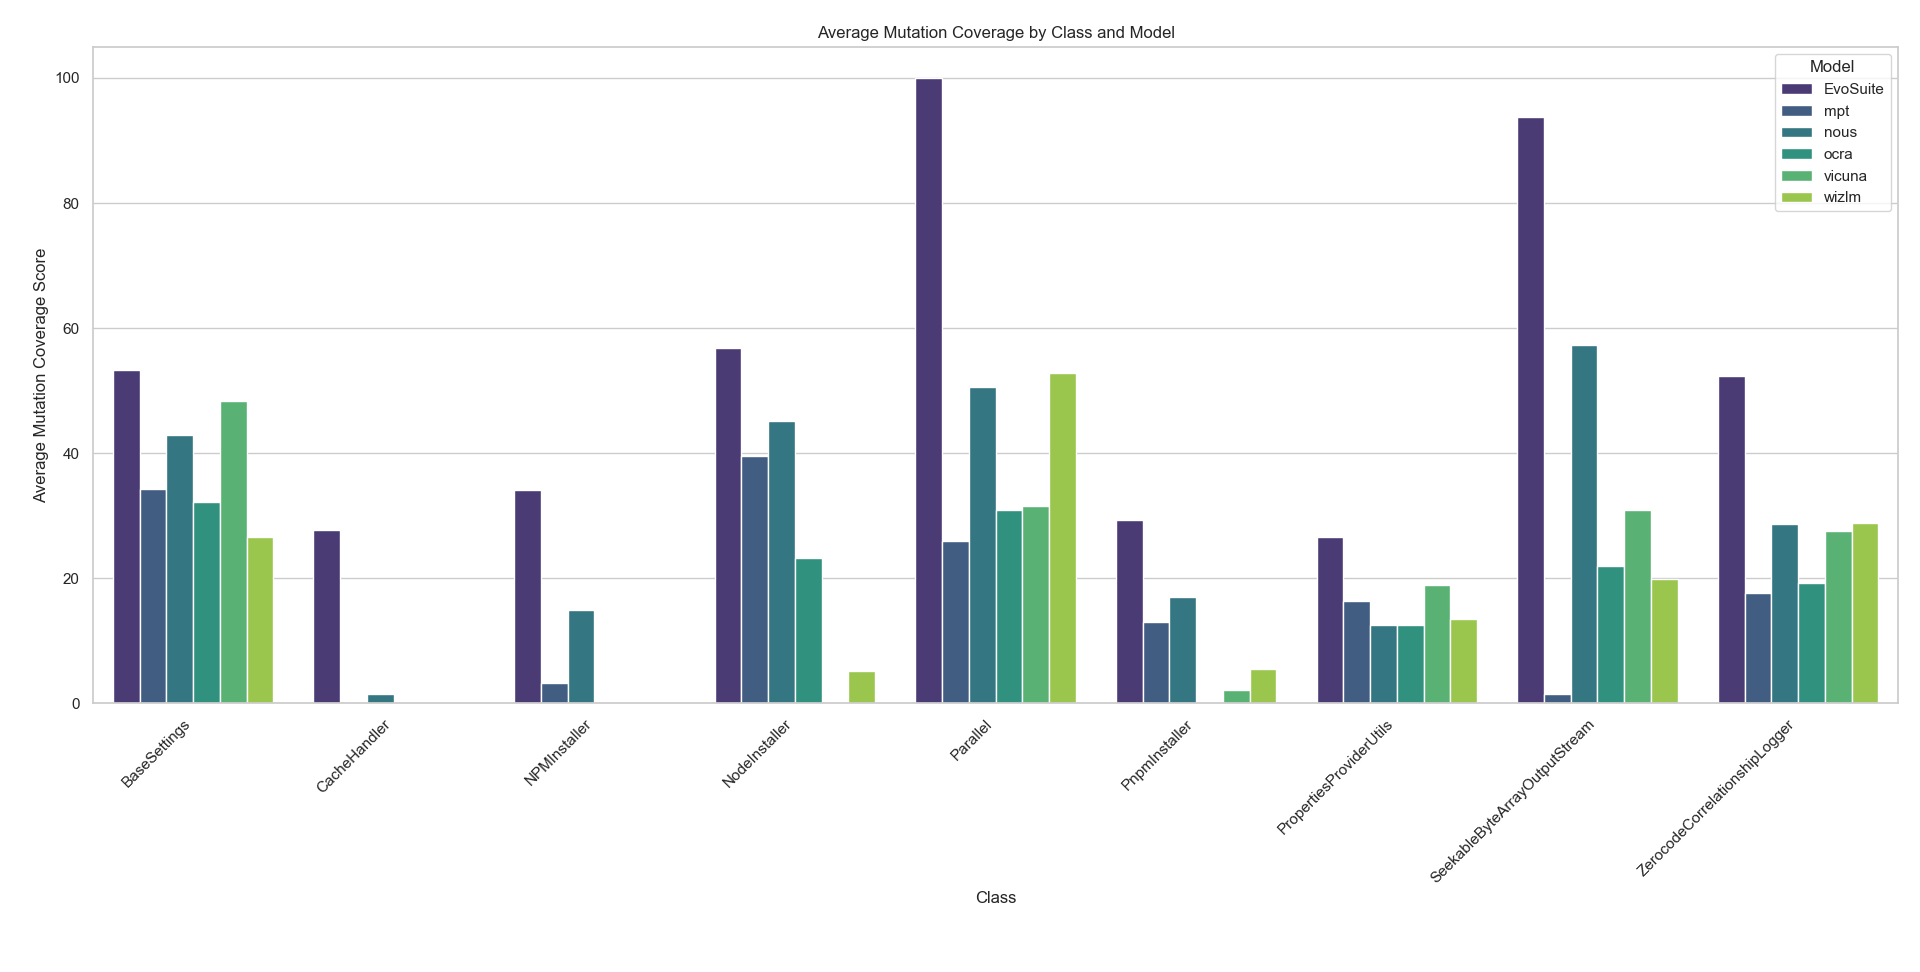
\includegraphics[width=1\textwidth]{images/mutation_coverage_avg.png}
\caption{Average Mutation Coverage by Class and Models}
\label{fig:mutation_coverage}
\end{figure}

\begin{figure}[H]
\centering
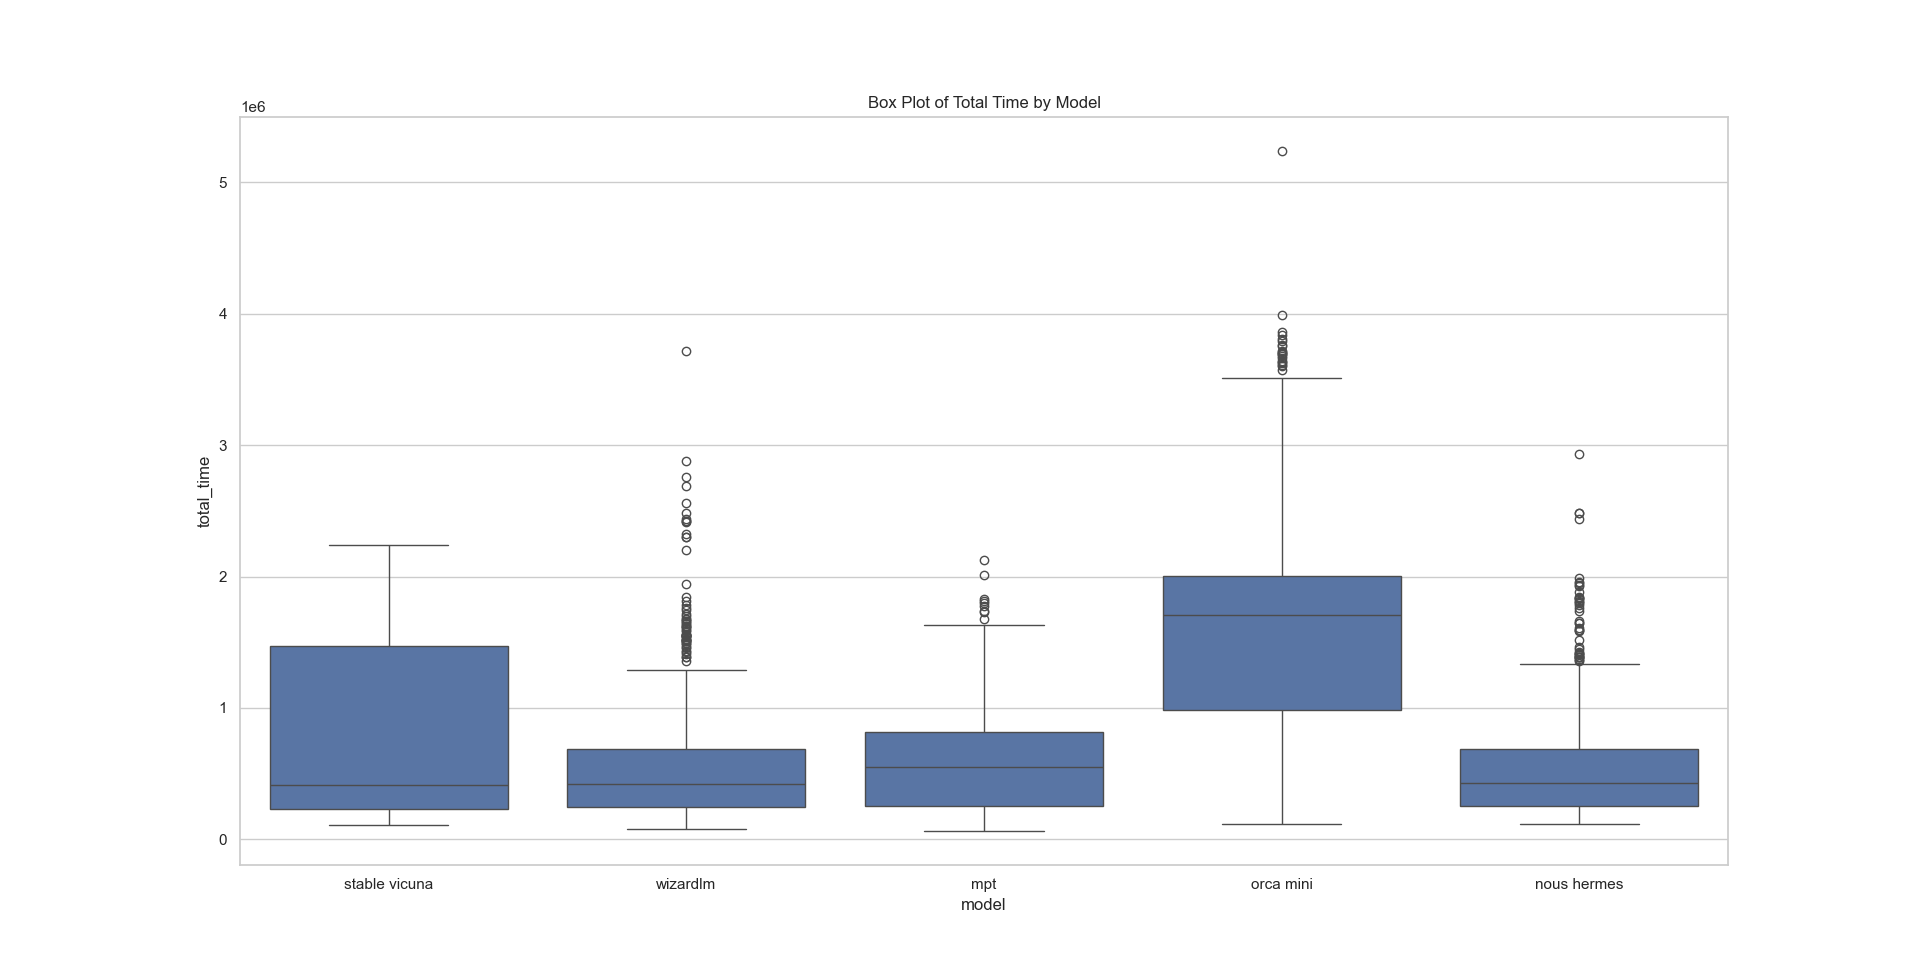
\includegraphics[width=1\textwidth]{images/time_by_model.png}
\caption{Total time taken by Models}
\label{fig:test_strength}
\end{figure}

\begin{figure}[H]
\centering
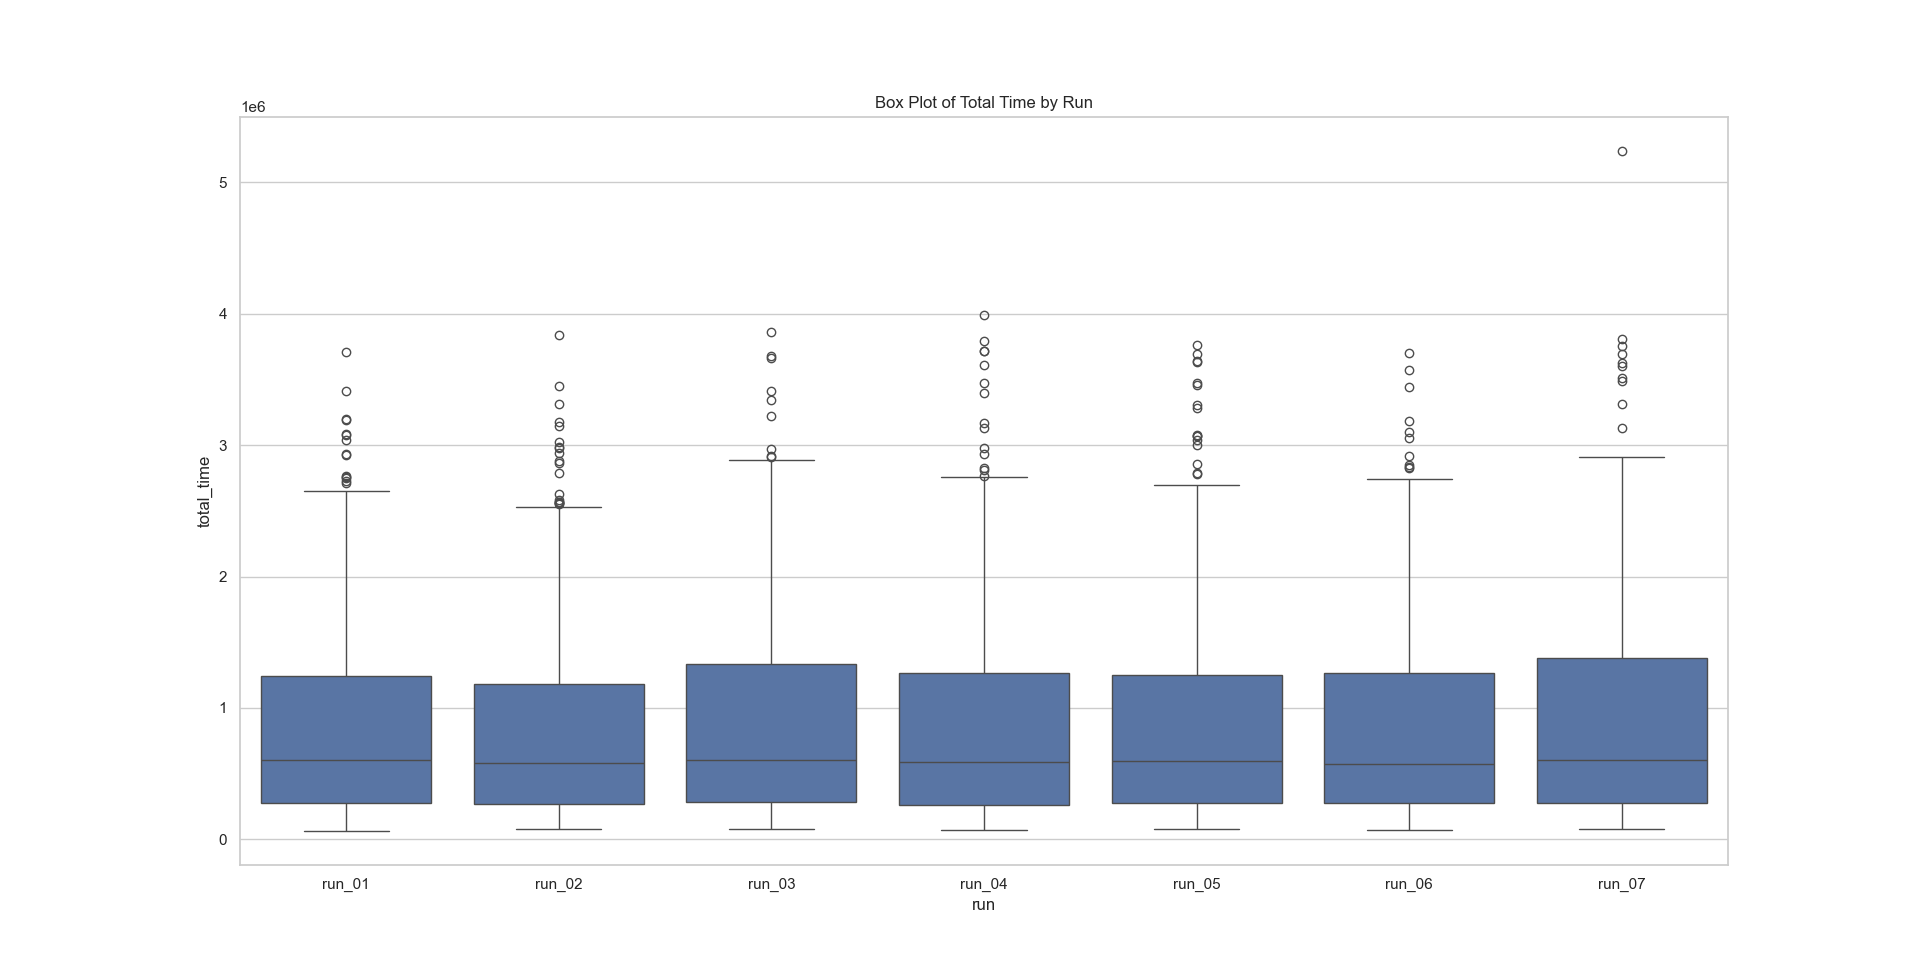
\includegraphics[width=1\textwidth]{images/time_by_runs.png}
\caption{Total time taken by each run}
\label{fig:test_strength}
\end{figure}

\begin{figure}[H]
\centering
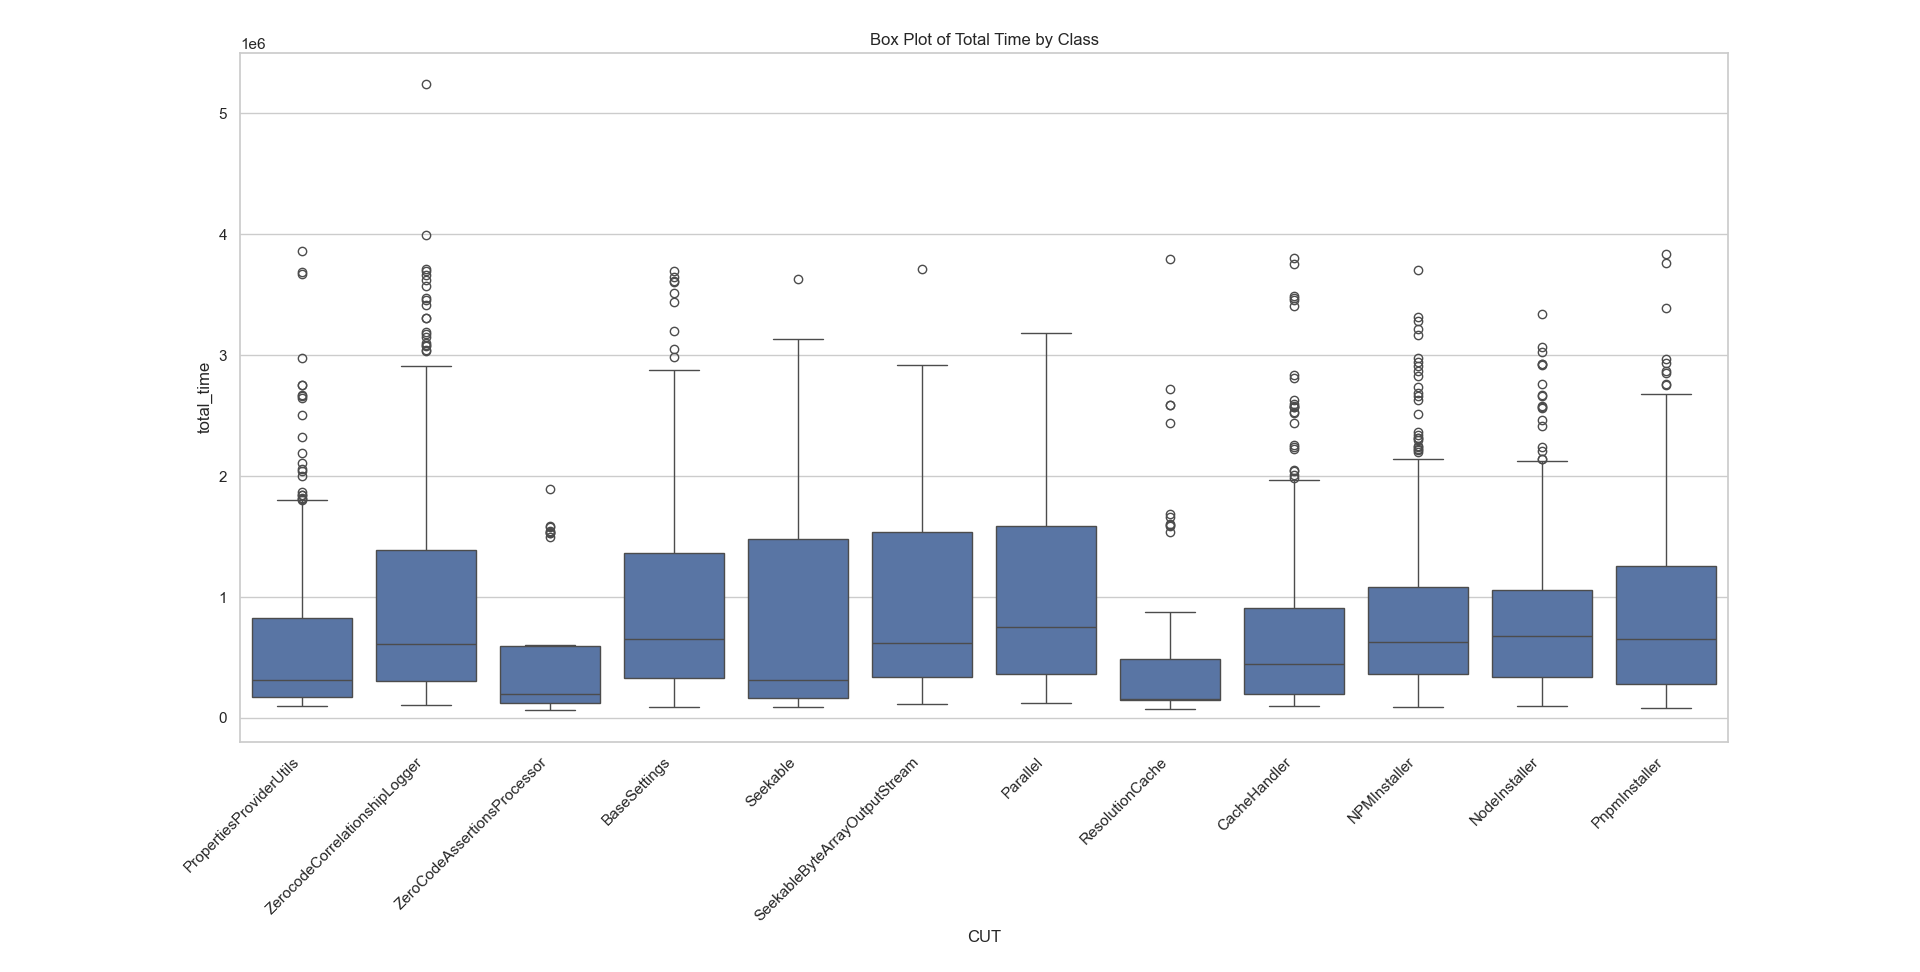
\includegraphics[width=1\textwidth]{images/total_time_by_class.png}
\caption{Total time taken by each class}
\label{fig:test_strength}
\end{figure}

\begin{figure}[H]
\centering
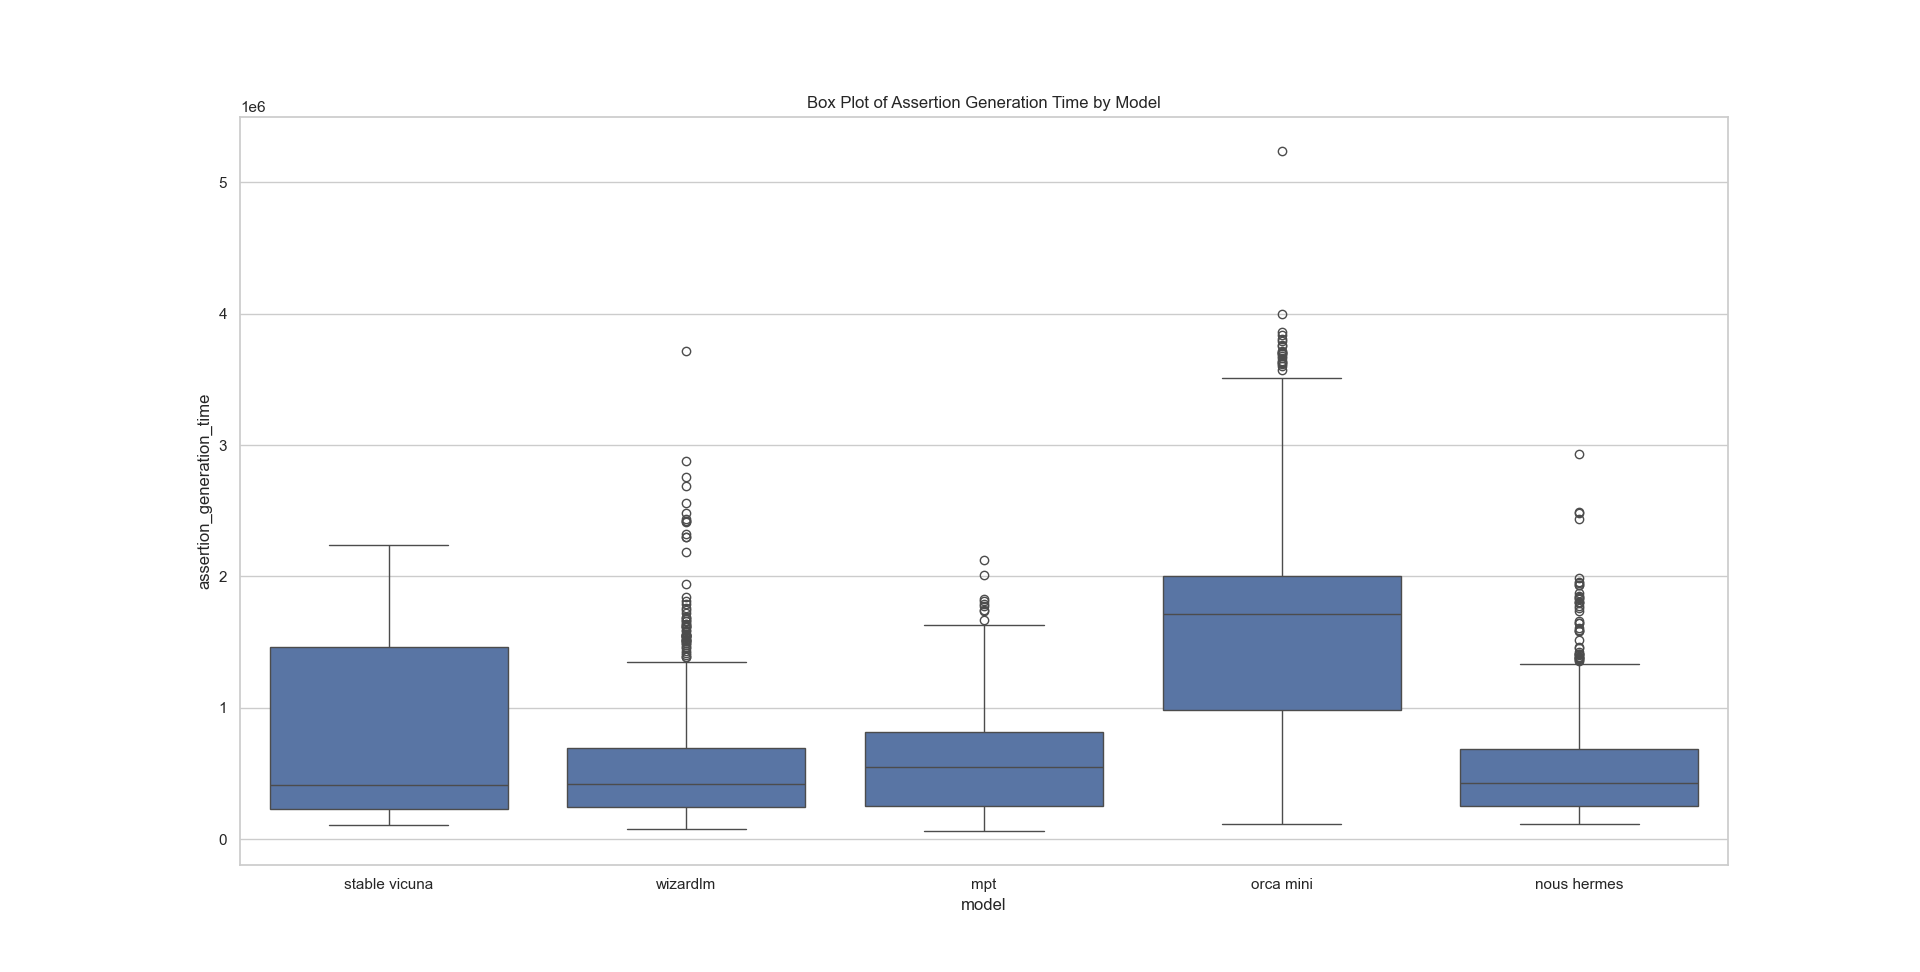
\includegraphics[width=1\textwidth]{images/assertion_time_by_model.png}
\caption{Assertion generation time taken by each model}
\label{fig:test_strength}
\end{figure}

\begin{figure}[H]
\centering
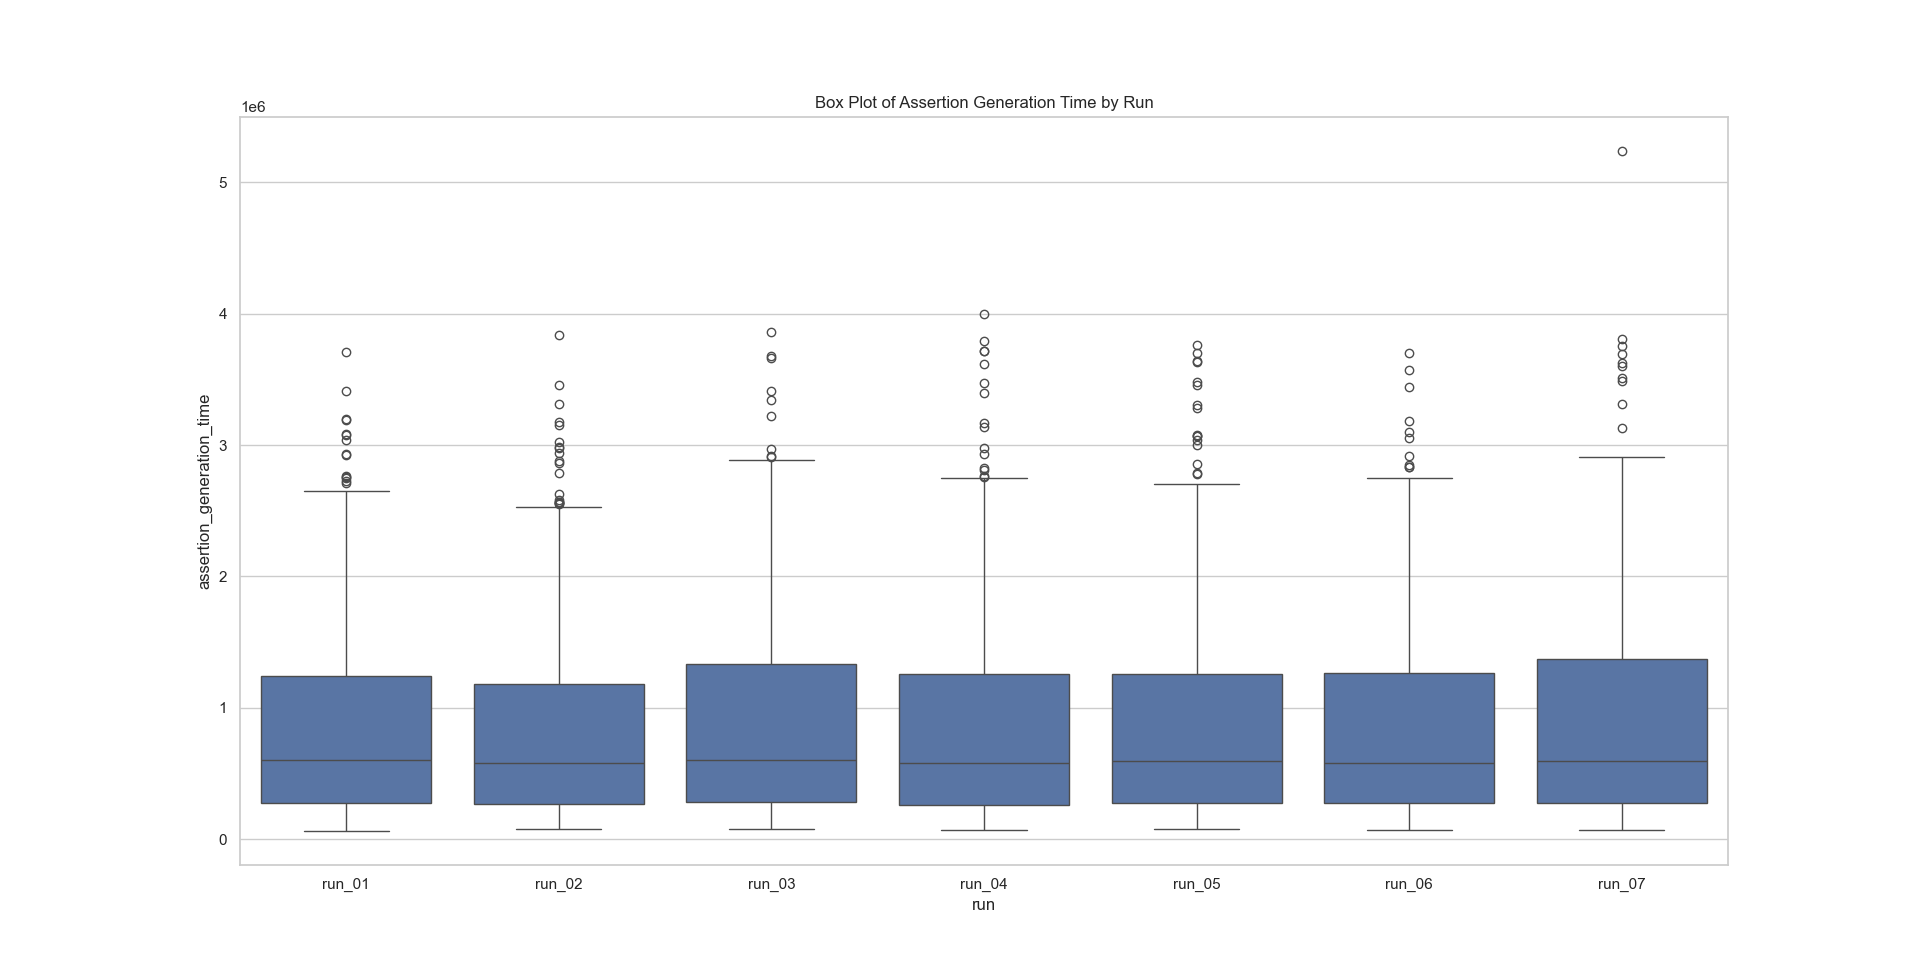
\includegraphics[width=1\textwidth]{images/assertion_time_by_runs.png}
\caption{Assertion generation time taken by each run}
\label{fig:test_strength}
\end{figure}

\begin{figure}[H]
\centering
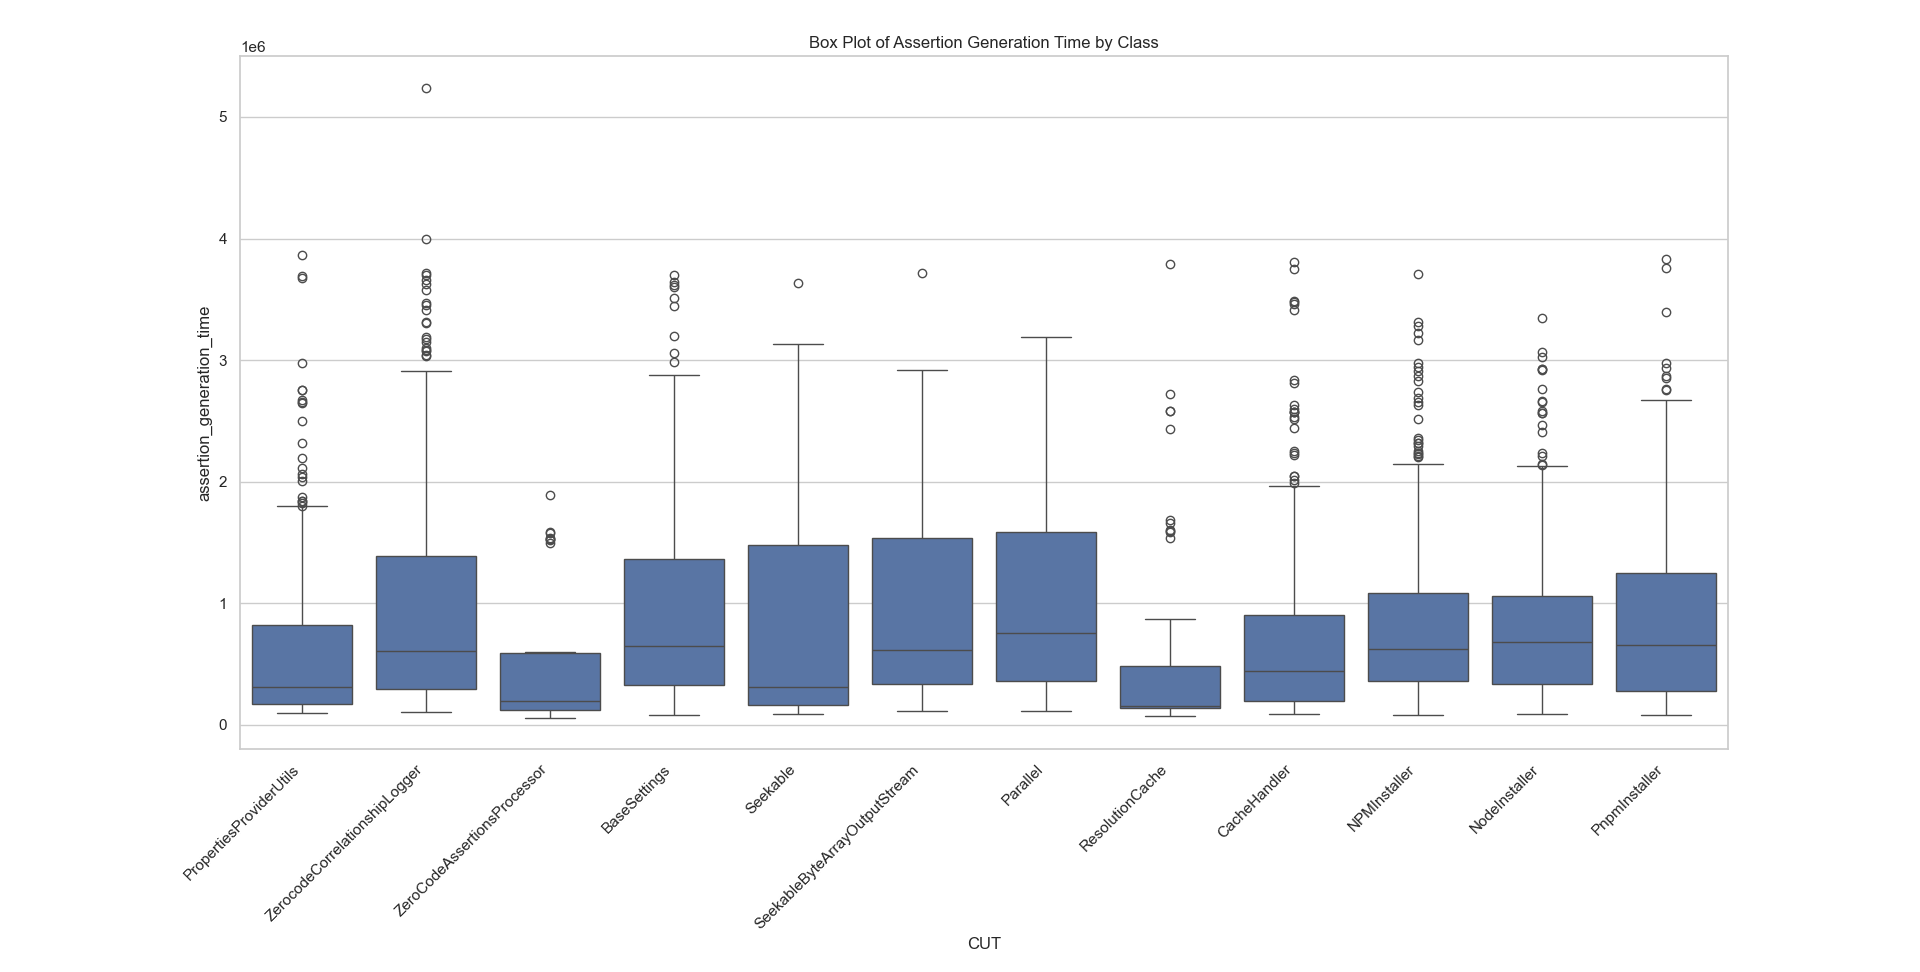
\includegraphics[width=1\textwidth]{images/assertion_time_by_class.png}
\caption{Assertion generation time taken by each class}
\label{fig:test_strength}
\end{figure}

\vspace{0.1 cm}
\subsection{RQ2: Efficiency of LLMs}
\label{sec:results_rq2}
\vspace{0.1 cm}

In this subsection, an overview of ...

\section{Threats to Validity}
\label{sec:t2v}
\vspace{0.2 cm}

The study acknowledges several potential threats to its validity.

\begin{enumerate}
    \item \textbf{Randomness in LLM Outputs:} One significant threat to the study's validity stems from the inherent randomness associated with Large Language Models (LLMs). The generated outputs are subject to variations based on the model's training conditions and prompt inputs, potentially impacting the reproducibility and consistency of results.

    \item \textbf{Generalizability to Diverse Datasets:} The study recognizes the potential limitation of generalizability to other datasets or programming languages. The findings, rooted in the analysis of Java projects from GitHub, may not extend seamlessly to different programming communities or languages, highlighting a domain-specific consideration.

    \item \textbf{Dataset-Induced Bias:} The dataset itself, composed of Java projects sourced from GitHub, introduces a possible bias reflective of the practices and characteristics specific to the Java programming community on this platform. This inherent bias could influence the study's conclusions and their applicability to broader software development contexts.

    \item \textbf{Concerns of Data Leakage:} In addressing concerns related to data leakage, the study takes precautionary measures by excluding candidate repositories that might appear in the pretraining corpus of the LLMs. This step aims to ensure the integrity of the evaluation process and prevent inadvertent leakage of information.

    \item \textbf{Selection Bias from Compilation and Execution Requirements:} The imposition of specific compilation and execution requirements, such as using Maven as the package manager and ensuring compatibility, introduces a potential source of selection bias. The study acknowledges the impact of these criteria on the composition of the chosen repositories, potentially affecting the representativeness of the dataset.

    \item \textbf{Evaluation Metrics Limitations:} The study recognizes the limitations of the chosen evaluation metrics and criteria. While these metrics provide a quantitative basis for assessment, they may not comprehensively capture the nuanced aspects of LLM-based test oracle generation. This acknowledgment indicates a need for a holistic understanding beyond the quantitative measures employed.
\end{enumerate}

These considerations collectively contribute to the study's robustness and transparency, providing insights into potential factors that may influence the interpretation and application of its findings.

\section{Discussion and Future Work}
\label{sec:discussion}
\vspace{0.2 cm}

In this section, a brief introduction to ... 

% \vspace{0.1 cm}
% \subsection{Subsection}
% \label{sec:transformers}
% \vspace{0.1 cm}

% In this subsection, an overview of ...

% \vspace{0.1 cm}
% \subsection{Another Subsection}
% \label{sec:automl}
% \vspace{0.1 cm}

% In this subsection, ...